

\begin{frame}[t,allowframebreaks]{Underfitting and overfitting -}

    Typically, 
    we we choose model parameters that reduce the training error, 
    and then test the model performance against the test set.
    \begin{itemize}
    \item 
    Under this process, 
    the expected value of the test error 
    is greater than (or equal to)  
    the expected value of the training error.
    \end{itemize}
 
    \vspace{0.2cm}
    
    A central challenge is to:
    \begin{itemize}
     \item {\bf reduce the training error}, \underline{and}
     \item {\bf reduce the gap between the training and test error}.
    \end{itemize}
 
    \vspace{0.2cm}   
 
    Failing on either of these goals, gives rise to common model pathologies:
    \begin{itemize}
      \item \index{underfitting}\Gls{underfitting}:
      Our model does not describe the training data well,
      and {\bf we cannot obtain a sufficiently small training error}.
      \item \index{overfitting}\Gls{overfitting}:
      We obtain a small training error,
      but {\bf our model does not generalize well} and  
      the training error is large. 
    \end{itemize}
 
    \framebreak
 
    %
    %
 
    \begin{center}
         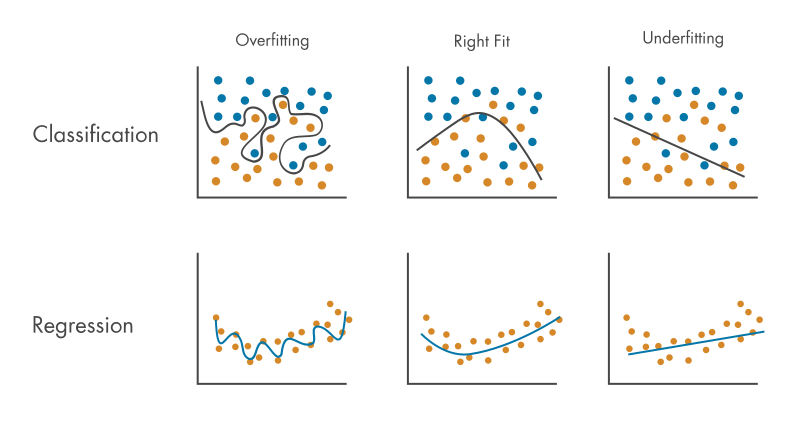
\includegraphics[width=1.0\textwidth]
             {./images/training_issues/over_and_underfitting_1.png}\\
         {\tiny 
             Illustrating overfitted and underfitted model pathologies.\\
             \color{col:attribution} 
             Schematic reproduced from \cite{MathWorks:Overfitting}.\\
         }
     \end{center}

     \framebreak
 
     Generally, \index{overfitting}\gls{overfitting} results, 
     amongst other reasons, from:
     \vspace{0.2cm}
     \begin{itemize}
        \item {\bf Insufficient training data set}.
        \begin{itemize}
            \item With limited data, one may find spurious patterns. 
        \end{itemize}    
        \item {\bf Various pathologies of the training set}.
        \begin{itemize}
            \item {\bf Selection bias} in the data collection process,
            or use of {\bf imbalanced training data} in classification tasks
            \item The presence of {\bf outliers in the training data},
            forcing the learning process to fit extremes rather than overall features.
        \end{itemize}    
        \item {\bf Too complex model architecture}.
        \begin{itemize}
            \item A model with too many parameters may simply memorize the
            data, instead of learning underlying features of the data.
            \item Models with over-engineered or noisy features.
        \end{itemize}    
        \item {\bf Lack of regularization} (see later in this lecture).
        \item {\bf Poorly tuned hyperparameters}, such as learning rate or batch size,
        or use of too many training epochs.

     \end{itemize}

     \framebreak
 
     On the other hand, \index{underfitting}\gls{underfitting} can be caused by:
     \vspace{0.2cm}
     \begin{itemize}
        \item a
     \end{itemize}
  
     %
     %
 
 \end{frame}
 